%----------------------------------------------------------------------------------------
%	PACKAGES AND DOCUMENT CONFIGURATIONS
%----------------------------------------------------------------------------------------

\documentclass[12pt,a4paper]{article}

\usepackage[version=3]{mhchem} % Package for chemical equation typesetting
\usepackage{siunitx} % Provides the \SI{}{} and \si{} command for typesetting SI units
\usepackage{graphicx} % Required for the inclusion of images
\usepackage{natbib} % Required to change bibliography style to APA
\usepackage{amsmath} % Required for some math elements 
\usepackage{geometry}
\usepackage{enumerate}
\usepackage{float}
\usepackage{subfigure}
\usepackage{pdfpages}
\usepackage{siunitx}
\usepackage{fancyhdr}
\usepackage{textcomp}
\usepackage{gensymb}

\includepdfset{pagecommand={\thispagestyle{fancy}}}%page number for pdf

\renewcommand{\labelenumi}{\alph{enumi}.} % Make numbering in the enumerate environment by letter rather than number (e.g. section 6)
\geometry{left=2cm,right=2cm,top=3cm,bottom=3cm}

%\usepackage{times} % Uncomment to use the Times New Roman font

%----------------------------------------------------------------------------------------
%	DOCUMENT INFORMATION
%----------------------------------------------------------------------------------------


\begin{document}

\begin{center}
~\\
\rule[0mm]{400pt}{0.5pt}
\Large{ \textsc{\newline\\UM-SJTU Joint Institute\\Physics Laboratory\\(Vp141)\\}}
\rule[0mm]{400pt}{0.5pt}
\Large{ \textsc{\newline\newline\newline\newline\newline\newline\\
Laboratory Report\\}}
\Large{\textsc{ \\ Exercise 5  \\ Damped and Driven Oscillations \\
Mechanical Resonance} }

\end{center}

\begin{description}
    \item[] 
    \item[] 
    \item[] 
    \item[] 
    \item[] 
    \item[]
    \item[]\qquad \qquad Name: Han Yibei \qquad ID:519370910123   \qquad    Group:11\\
    \item[]\qquad \qquad Date: \today
\end{description}

\newpage

%----------------------------------------------------------------------------------------
%	SECTION 1
%----------------------------------------------------------------------------------------

\section{Introduction}

The objective of this experiment is to use the Pohl resonator to study damped and driven oscillations in mechanical systems. We will study the property of mechanical resonance by analyzing the figure based on our experimental data.

\section{Theoratical background}
If a force which varies periodically is exerted on a damped harmonic oscillator, the motion is called forced (or driven) oscillations. Suppose the form of the driving force is 
\begin{equation}
    F=F_0cos\omega t
\end{equation} 
Where $F_0$ is the amplitude and $\omega$ is the angular frequency. \par 
When the oscillator reaches the steady state, its angular frequency will be the same as $\omega$. \par 
The amplitude of the steady-state oscillation depends on the relationship between the natural angular frequency and the driving frequency, and the damping coefficient. When the amplitude becomes quite large, the phenomenon is called mechanical resonance. \par 
There will be a phase lag between the driving force and the displacement from equilibrium of the oscillating particle. When $\omega$ equals the natural frequency, the phase lag is $\pi/2$. \par 
In this experiment, we will use angular counterparts to replace the linear quantities. \par 
When a driving torque $\tau_dr=\tau_0 cos\omega t$ and a damping torque $\tau_f=-b\frac{d\theta}{dt}$ and a restoring force acted upon the balance wheel, its equation of motion is
\begin{equation}
    I\frac{d^2\theta}{dt^2}=-k\theta-b\frac{d\theta}{dt}+\tau_0cos\omega t
\end{equation}
where $I$ is the moment of inertia of the balance wheel, $\tau_0$ is the amplitude of the driving torque, and $\omega$ is angular frequency of the driving torque. \par 
Introducing the following symbols $ {ω_0}^2=\frac{k}{I}, 2\beta=\frac{b}{I},\mu=\frac{\tau_0}{I}$ ,Eq.2 can be written as:
\begin{equation}
    I\frac{d^2\theta}{dt^2}+2\beta\frac{d\theta}{dt}+{\omega_0}=\mu cos\omega t
\end{equation}

\begin{equation}
    \theta(t)=\theta_{tr}(t)+\theta_(st)cos(\omega t+\phi)
\end{equation}

where $\theta_{tr}$ denotes the transient solution and
\begin{equation}
  \theta_{st}=\frac{\mu}{\sqrt{({\omega_0}^2-\omega^2)^2+4\beta^2\omega^2}} 
\end{equation} 
\par

The phase shift $\phi$ satisfies the equation:
\begin{equation}
    tan\phi=\frac{2\beta\omega}{\omega^2-{\omega_0}^2}
\end{equation}
where $-\pi\leq\phi\leq 0$, which is independent of the initial conditions. \par 
By finding the maximum value of $\theta_{st}$, we can find the resonance angular frequency $\omega=\omega_{res}=\sqrt{{\omega_0}^2-2\beta^2}$ (7), and the corresponding amplitude is $\theta_{res}=\theta_{st}(\omega_{res})=\frac{\mu}{2\beta\sqrt{{\omega_0}^2-\beta^2}})$ (8). \par 
The dependence of the amplitude and the phase on the driving angular frequency is shown in figure 3. When damping increases, the resonance frequency will move away from the natural frequency to a smaller value and the amplitude of the steady-state oscillation decreases.


\section{Apparatus}
The experimental setup is shown in figure 3 and 4.

The BG-2 Pohl resonator consists of two main parts: a vibrometer (Figure 3) and a control box(Figure 4). The scroll spring provides an elastic restoring torque so that the wheel can rotate about an equilibrium state.
There are notches on the edge of the wheel, and one of them is deeper than the others. When this notch passes the photoelectric detector(1), the period of oscillations can be measured. The amplitude can also be measured by counting the notches and will be displayed. Another photoelectric detector(11) is set above the turntable and can measure the period of the driving force. When the Period Selection switch is at position “1”, a single oscillation period will be displayed; when it is at position “2”, the time of 10 period will be displayed. \par 
The damping comes from the pair of coils at the bottom of the supporting frame. When the coils carry current, the electromagnetic force will serve as the damping torque. Its magnitude can be changed by changing the current. The Damping Selection knob can be used to change the current. \par 
A motor and an electric wheel are used to drive the wheel.\par 
As for the control box, a Period Selection switch and a Period of Driving Force can be used to control the speed of the motor precisely.\par 
To measure the phase shift, the glass turntable with an angle scale and a strobe light are used. When the deep notch passes the detector, a line on the scale will be highlighted and can be read.\par 

The information of each measuring scale is shown in Table 1.

\begin{table}[H]
    \centering
    \begin{tabular}{|c|c|c|c|}
    \hline
    apparatus& range & resolution & uncertainty \\ \hline
    Vibrometer-period    & /& 0.001s& $\pm$0.001s\\ \hline
    Vibrometer-angle& 0-180\degree & 1\degree    & $\pm$1\degree\\ \hline
    Vibrometer-amplitude & /& 1\degree    & $\pm$1\degree\\ \hline
    \end{tabular}
    \caption{Information of Each Measuring scale}
    \end{table}


 
\section{Measurement}
\subsection{Natural Angular Frequency}
\begin{enumerate}
    \item Rotate the wheel to a degree of about 90\degree and release it, and record the time of 1 period.
    \item Repeat step a and record 4 sets of data and calculate the natural angular frequency.
\end{enumerate}

\subsection{Damping Coefficient}
\begin{enumerate}
    \item  Turn the Damping mode to 2 and do not change it.
    \item Rotate the wheel to a degree of about 90\degree and release it, and record the value of amplitude each period and the time of 10 intervals.
    \item The damping coefficient can be calculated using the equation 
$\beta=\frac{1}{5T}ln\frac{\theta_i}{\theta_{i+5}}$
    where T is the average period
\end{enumerate}

\subsection{$\theta_{st}$ vs. $\omega$ and $\phi$ vs. $\omega$ Characteristics of Forced Oscillations}
\begin{enumerate}
    \item Choose damping mode 2 and set the speed of the motor.
    \item Wait until the oscillation reaches its steady state where the amplitude doesn’t change. Record the amplitude $\theta_{st}$, the period T and the phase shift $\phi$.
    \item Repeat step 2 for 15-20 times. Change the speed of motor slowly and collect more data when phase shift is near $\pi/2$. 
    \item Choose Damping Selection 1 or 3. Repeat the above steps. 
    \item Plot the $\theta_{st}$ characteristics, set $\omega/\omega_0$ the horizontal axis and $\theta_{st}$ the vertical axis. Plot the data of two different modes on the same graph.
    \item Plot the $\phi$ characteristics, set $\omega/\omega_0$ the horizontal axis and $\phi$ the vertical axis. Plot the data of two different modes on the same graph.
    
\end{enumerate}

\section{Result}
\subsection{Natural Angular Frequency}
\begin{table}[H]
    \centering
    \begin{tabular}{|c|c|}
    \hline
& T{[}s{]}$\pm$0.001{[}s{]} \\ \hline
    1 & 1.556  \\ \hline
    2 & 1.556   \\ \hline
    3 & 1.556   \\ \hline
    4 & 1.556   \\ \hline
    \end{tabular}
    \caption{Measurement of the natural frequency}
\end{table}
From table 2 we get the average value of the time of one period:
$$\overline{T}=\frac{1}{4}\sum^4_{n=1}T_n=\frac{1.556+1.556+1.556+1.556}{4}=1.556\pm0.001s$$
The natural frequency can be calculated as $\omega_0=\frac{2\pi}{T}=4.038\pm 0.003 rad/s$

\subsection{Damping Coefficient}
\begin{table}[h]
    \centering
    \begin{tabular}{|c|c|c|c|c|}
    \hline
    \multicolumn{2}{|c|}{Amplitude{[}\textdegree{]}$\pm$ 1{[}\textdegree{]}} & \multicolumn{2}{c|}{Amplitude{[}\textdegree{]}$\pm$ 1{[}\textdegree{]}} & $\ln{(\theta_i/\theta_{i+5})}$ \\ \hline
    $ \theta_0 $& 88   & $ \theta_5   $& 55 & 0.470
    \\ \hline
    $ \theta_1 $& 80   & $  \theta_6   $    & 50 & 0.470
    \\ \hline
    $ \theta_2  $& 73   & $  \theta_7     $  & 46 & 0.462
    \\ \hline
    $ \theta_3   $    & 66   & $    \theta_8   $  & 42 & 0.452
    \\ \hline
    $ \theta_4   $    & 60   & $ \theta_9     $   & 38 & 0.457
    \\ \hline
    \multicolumn{4}{|c|}{The average value of ln($\theta_i/\theta_{i+5}$)}& 0.462
    \\ \hline
    \end{tabular}
    \caption{Measurement of the damping coefficient}
\end{table}

The measured time of a period 10T=15.550s$\pm$0.001s, so T=1.5550$\pm$0.0001s \par 
The last data in table 3 is calculated by
$$\overline{ln(\theta_i/\theta_{i+5})}=\frac{1}{5}\sum^4_{i=0}ln(\theta_i/\theta_{i+5})=\frac{0.470+0.470+0.462+0.452+0.457}{5}=0.46\pm 0.03$$
Use the equation $\beta=\frac{1}{5T}ln(\theta_i/\theta_{i+5})=\frac{1}{5\times 1.5550}\times 0.462=0.059\pm 0.004s^{-1}$

\subsection{$\theta_{st}$ vs. $\omega$ and $\phi$ vs. $\omega$ Characteristics of Forced Oscillations}

\subsubsection{Damping Selection 2}

We can found that $\frac{\omega}{\omega_0}=\frac{T_{natural}}{T_{driven}}$ and $T_{natural}=1.556\pm0.001s$

\begin{table}[H]
    \centering
    \begin{tabular}{|c|c|c|c|c|}
    \hline
    T[s]$\pm$0.001[s]& $\omega/\omega_0$ & uncertainty for $\omega/\omega_0$ & $\phi${[}\degree{]}$\pm$1{[}\degree{]} & $\theta${[}\degree{]}$\pm$1{[}\degree{]} \\ \hline
    1.474 & 1.0556& 0.0013& -164& 34   \\ \hline
    1.486 & 1.0471& 0.0012& -161& 40   \\ \hline
    1.501 & 1.0366& 0.0012& -157& 49   \\ \hline
    1.511 & 1.0298& 0.0012& -152& 59   \\ \hline
    1.524 & 1.0210& 0.0012& -145& 76   \\ \hline
    1.533 & 1.0150& 0.0012& -135& 90   \\ \hline
    1.541 & 1.0097& 0.0012& -123& 109  \\ \hline
    1.553 & 1.0019& 0.0012& -100& 128  \\ \hline
    1.556 & 1.0000& 0.0012& -92& 130  \\ \hline
    1.558 & 0.9987& 0.0012& -89& 130  \\ \hline
    1.560  & 0.9974& 0.0012& -84& 129  \\ \hline
    1.564 & 0.9949& 0.0012& -74& 126  \\ \hline
    1.573 & 0.9892& 0.0012& -58& 112  \\ \hline
    1.583 & 0.9829& 0.0012& -47& 93   \\ \hline
    1.592 & 0.9774& 0.0012& -38& 78   \\ \hline
    1.605 & 0.9695& 0.0012
    & -30& 63   \\ \hline
    1.619 & 0.9611& 0.0011
    & -24& 51   \\ \hline
    1.628 & 0.9558& 0.0011
    & -21& 46   \\ \hline
    1.642 & 0.9476& 0.0011
    & -18& 39   \\ \hline
    \end{tabular}
    \caption{$\theta_{st}$ vs. $\omega$ and $\phi$ vs. $\omega$ Characteristics of 5.3.1}
    \end{table}

\subsubsection{Damping Selection 3}
    \begin{table}[H]
  \centering
  \begin{tabular}{|c|c|c|c|c|}
  \hline
  T[s]$\pm$0.001[s]& $\omega/\omega_0$ & uncertainty for $\omega/\omega_0$ & $\phi${[}\degree{]}$\pm$1{[}\degree{]} & $\theta${[}\degree{]}$\pm$1{[}\degree{]} \\ \hline
  1.476   & 1.0542& 0.0013   & -164  & 35\\ \hline
  1.487   & 1.0464& 0.0012   & -162  & 40\\ \hline
  1.501   & 1.0366& 0.0012   & -158  & 50\\ \hline
  1.508   & 1.0318& 0.0012   & -155  & 56\\ \hline
  1.521   & 1.0230& 0.0012   & -149  & 72\\ \hline
  1.529   & 1.0177& 0.0012   & -141  & 88\\ \hline
  1.541   & 1.0097& 0.0012   & -125  & 114\\ \hline
  1.552   & 1.0026& 0.0012   & -101  & 133\\ \hline
  1.553   & 1.0019& 0.0012   & -99   & 137\\ \hline
  1.555   & 1.0006& 0.0012   & -93   & 137\\ \hline
  1.558   & 0.9987& 0.0012   & -88   & 138\\ \hline
  1.559   & 0.9981& 0.0012   & -84   & 137\\ \hline
  1.564   & 0.9949& 0.0012   & -74   & 130\\ \hline
  1.571   & 0.9905& 0.0012   & -60   & 122\\ \hline
  1.581   & 0.9842& 0.0012   & -48   & 99\\ \hline
  1.594   & 0.9762& 0.0012   & -36   & 76\\ \hline
  1.606   & 0.9689& 0.0012   & -28   & 62\\ \hline
  1.618   & 0.9617& 0.0011   & -23   & 52\\ \hline
  1.629   & 0.9552& 0.0011   & -20   & 45\\ \hline
  1.643   & 0.9470& 0.0011   & -17   & 39\\ \hline
  \end{tabular}
  \caption{$\theta_{st}$ vs. $\omega$ and $\phi$ vs. $\omega$ Characteristics of 5.3.2}
  \end{table}

\subsection{Comparing Figures}
   
\begin{figure}[H]
    \begin{minipage}[t]{9cm}
    \centering
    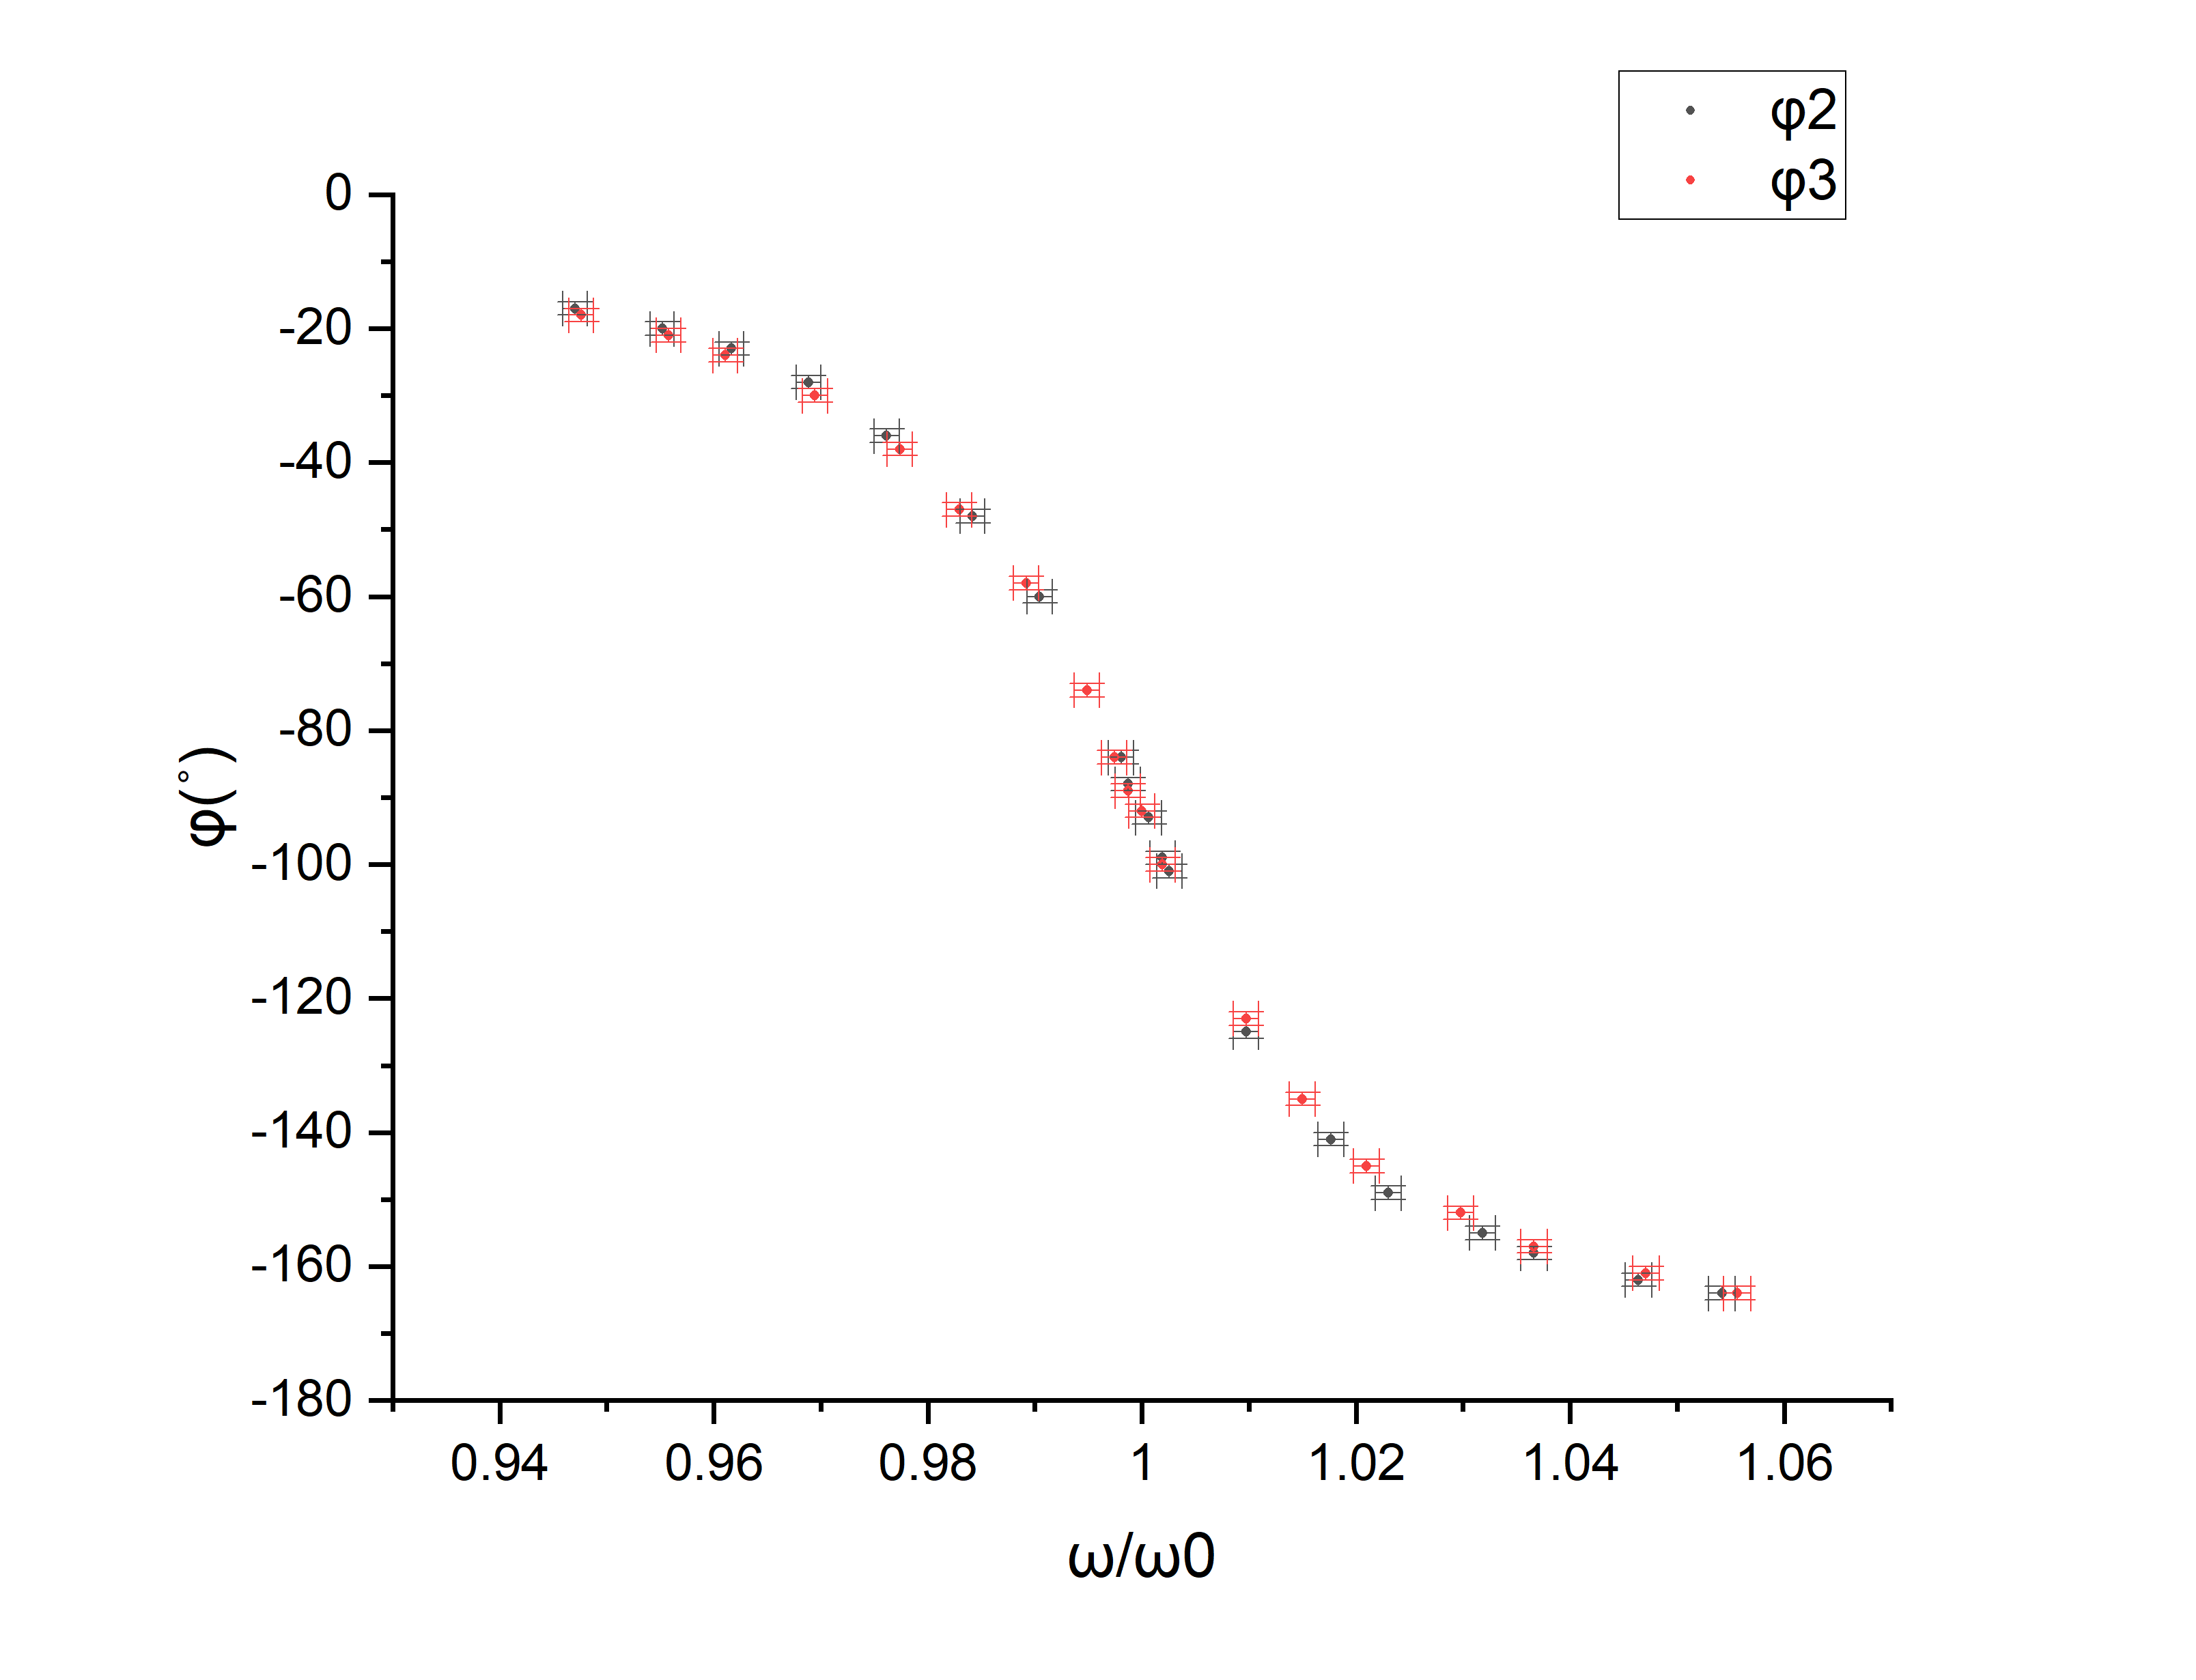
\includegraphics[width=9cm]{phi.png}
    \caption{$\phi$ v.s. $\omega/\omega_0$ characteristics}
    \end{minipage}
    \begin{minipage}[t]{9cm}
    \centering
    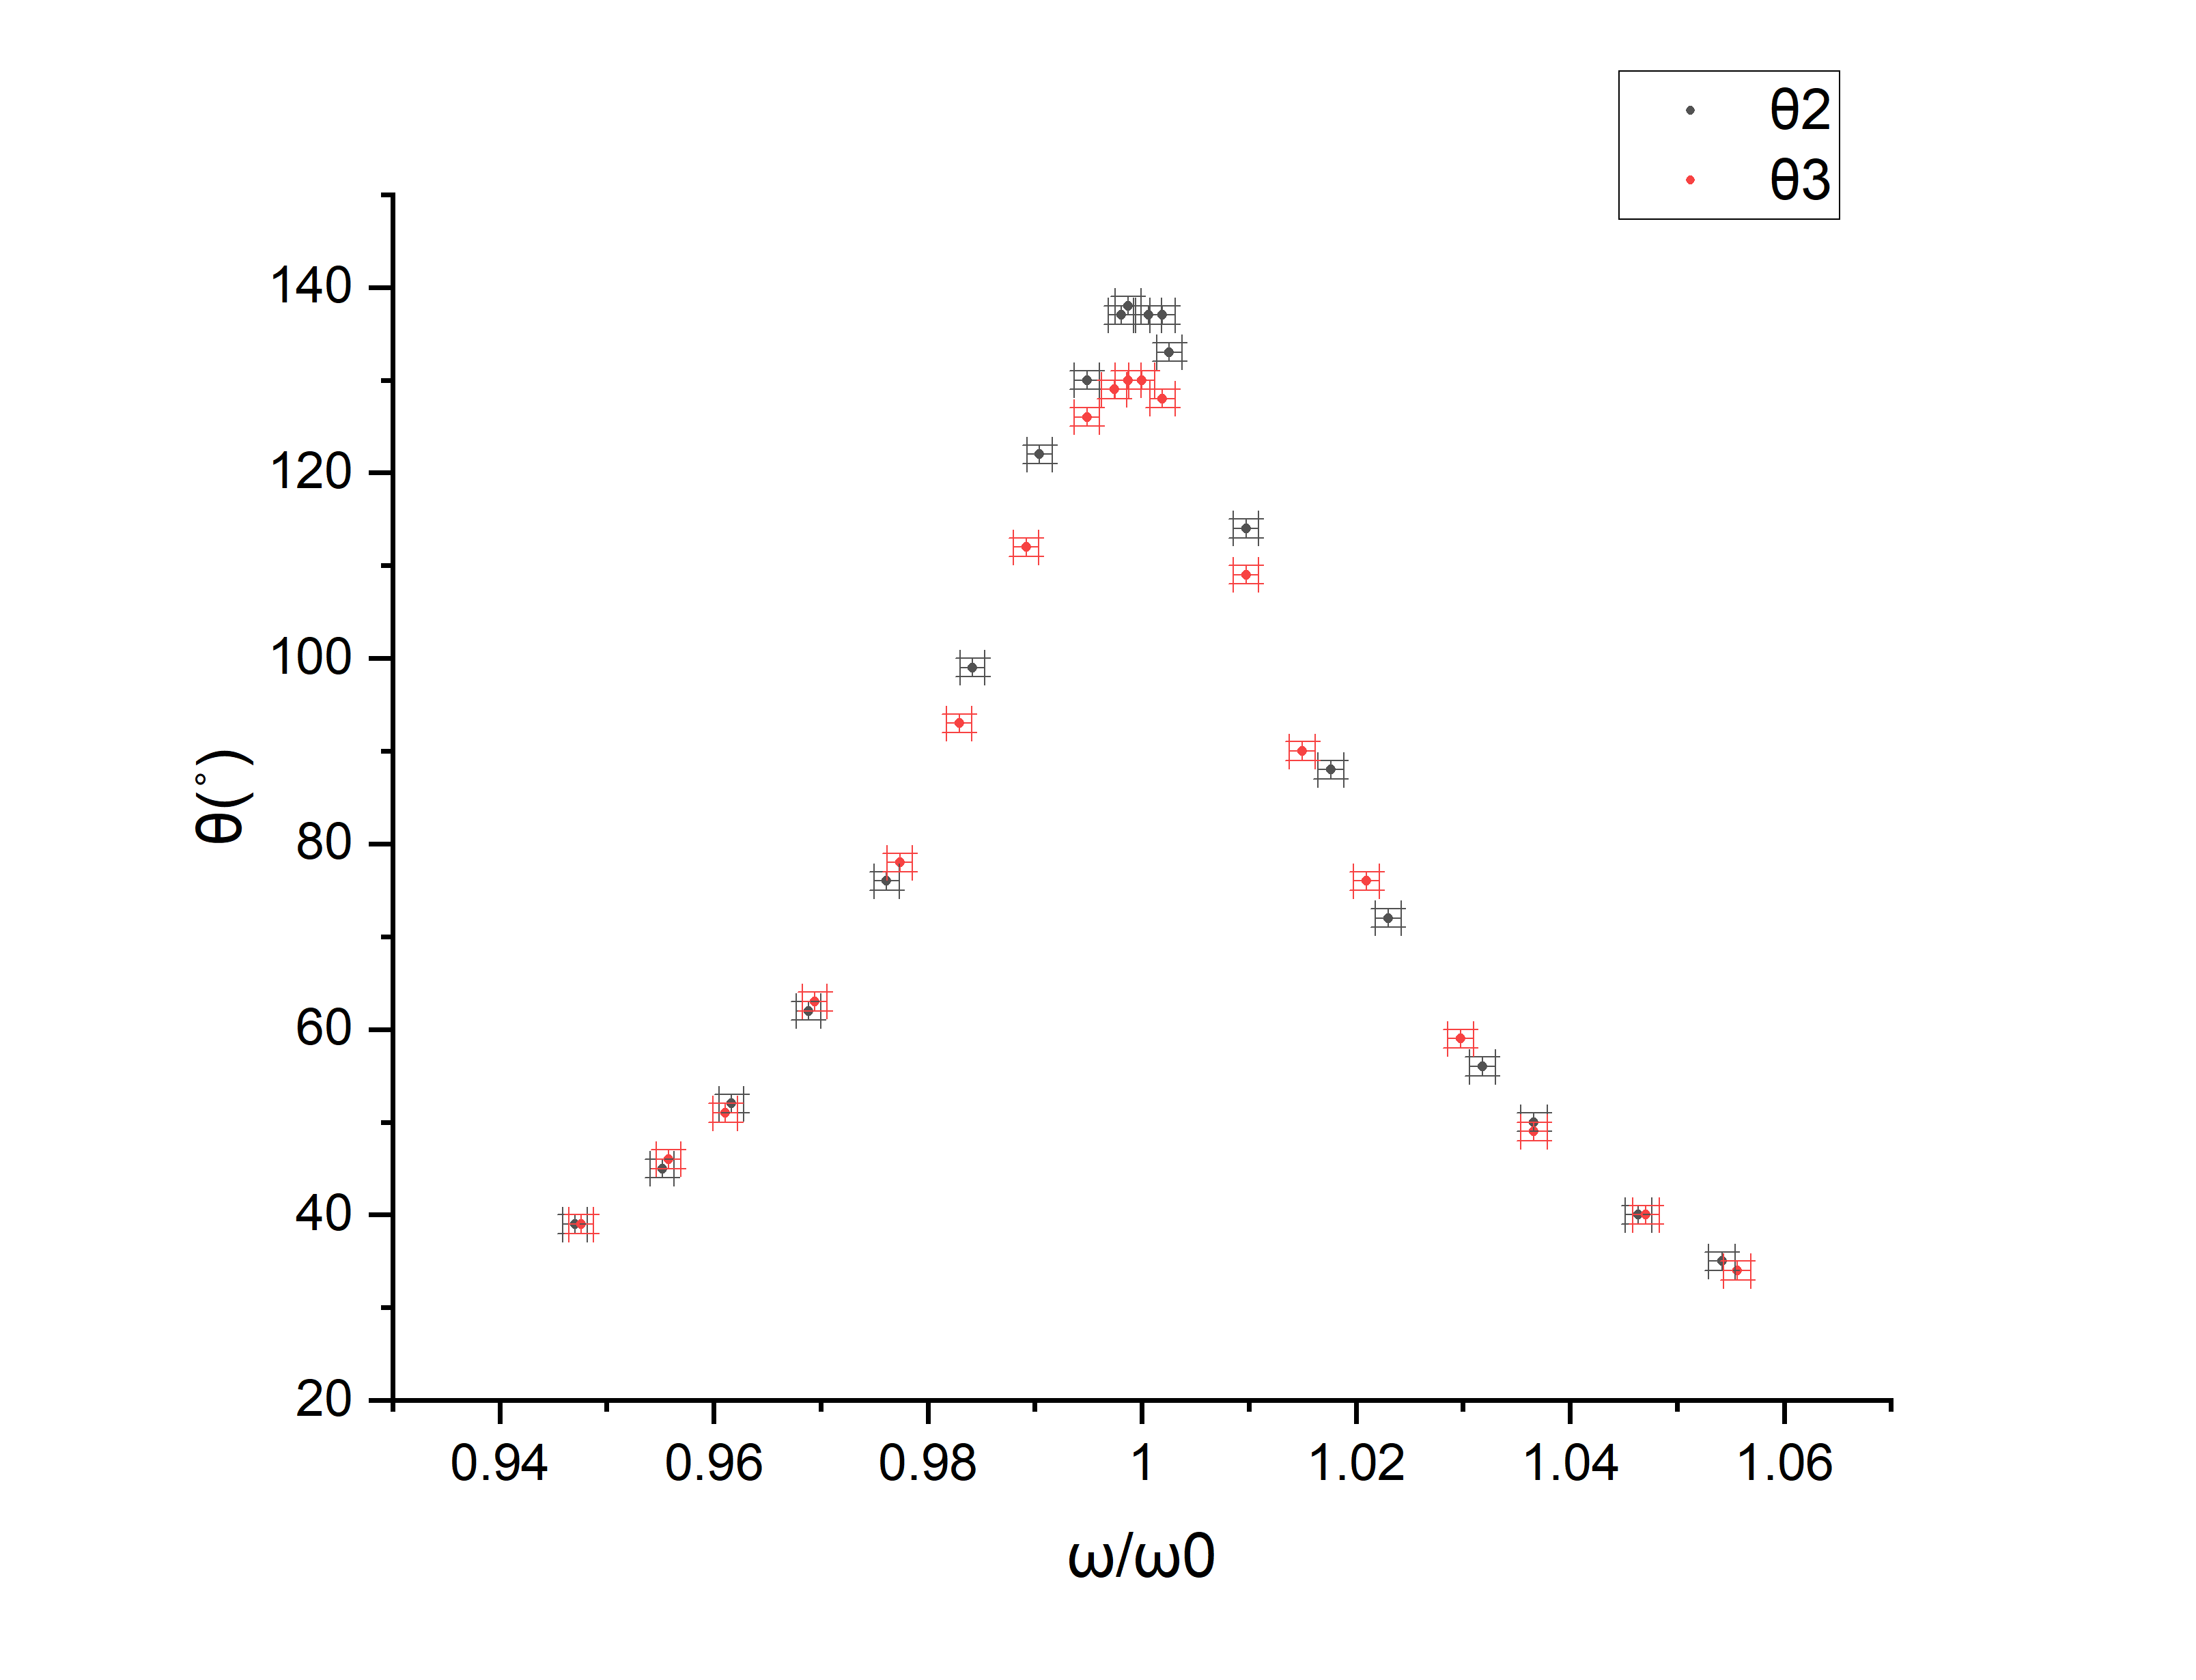
\includegraphics[width=9cm]{theta.png}
    \caption{$\theta_{st}$ v.s. $\omega/\omega_0$ characteristics}
    \end{minipage}
\end{figure}

From the graph of $\theta_{st}$ we can see when $\omega/\omega_0$ is close to 1, the amplitude reaches its maximum, which shows that the wheel is at mechanical resonance. Also, from the higher points, we can find that $\beta_2<\beta_3$. \par 
Also, from the graph of $\phi$, we could find that the slope reaches its maximum when $\omega/\omega_0$ approximately equals 1 and $\beta_2<\beta_3$.  

\section{Conclusion and Discussion}
\subsection{Conclusions}
The natural frequency is 4.038$\pm$0.003$rad/s$. \par 
The damping coefficient is 0.059$\pm$0.04$s^-1$. \par
The relative uncertainties are 0.06\% and 0.07\% respectively, which are small enough to prove the accuracy of our measurements.\par 
From the $\theta-\omega/\omega_0$  figure we can conclude:
\begin{itemize}
    \item When the driving frequency is near the natural frequency, the steady-state amplitude will peak
    \item When damping increases, the resonance frequency will move away from the natural frequency to a smaller value and the amplitude of the steady-state oscillation decreases.
\end{itemize}
From the $\phi-\omega/\omega_0$ figure we can conclude:
\begin{itemize}
    \item The phase lag becomes larger when the driving frequency increases.
    \item When the driving frequency is near the natural frequency, the phase lag is near $\pi/2$, and there’s a sharp change in the phase lag within this range
\end{itemize}

\subsection{Discussions}
The errors might exist because:
\begin{itemize}
    \item The air drag and friction inside the wheel will disturb the oscillation.
    \item It’s hard to tell whether the oscillation has reached its steady state because the amplitude might be changing even if we think that it stays still.
    \item	When reading the phase lag, the instantaneous flash light is hard to catch because it disappears too fast. Also, we observed that the phase lag was not stable, switching between two adjacent values. Therefore, the reading of phase lag might be inaccurate.
\end{itemize}

\subsection{Improvements}
\begin{itemize}
    \item 	The accuracy of the device can be improved. As can be seen from table 4 and 5, some value of $\theta$ are the same due to the limitation of the precision of the vibrometer. This will result in a flat slope on the figure. It will be better if the minimum scale of value can be small enough to distinguish these data.
    \item Use another method to read the phase lag since reading when the light flashes is not optimal.
\end{itemize}


\newpage
{\LARGE\textbf{APPENDIX}}
\setcounter{section}{0}
\renewcommand\thesection{\Alph{section}}

\section{Implementary Figures}
\begin{figure}[H]
    \centering
    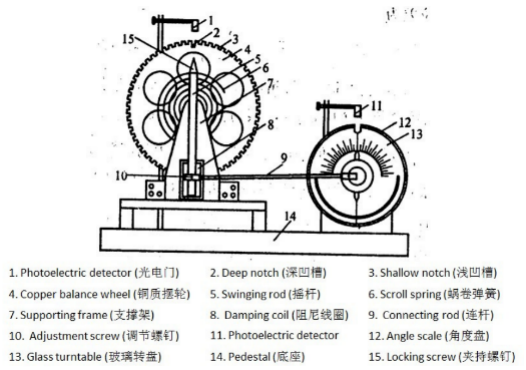
\includegraphics[width=10cm]{vibrometer.png}
    \caption{The vibrometer}
\end{figure}

\begin{figure}[H]
    \centering
    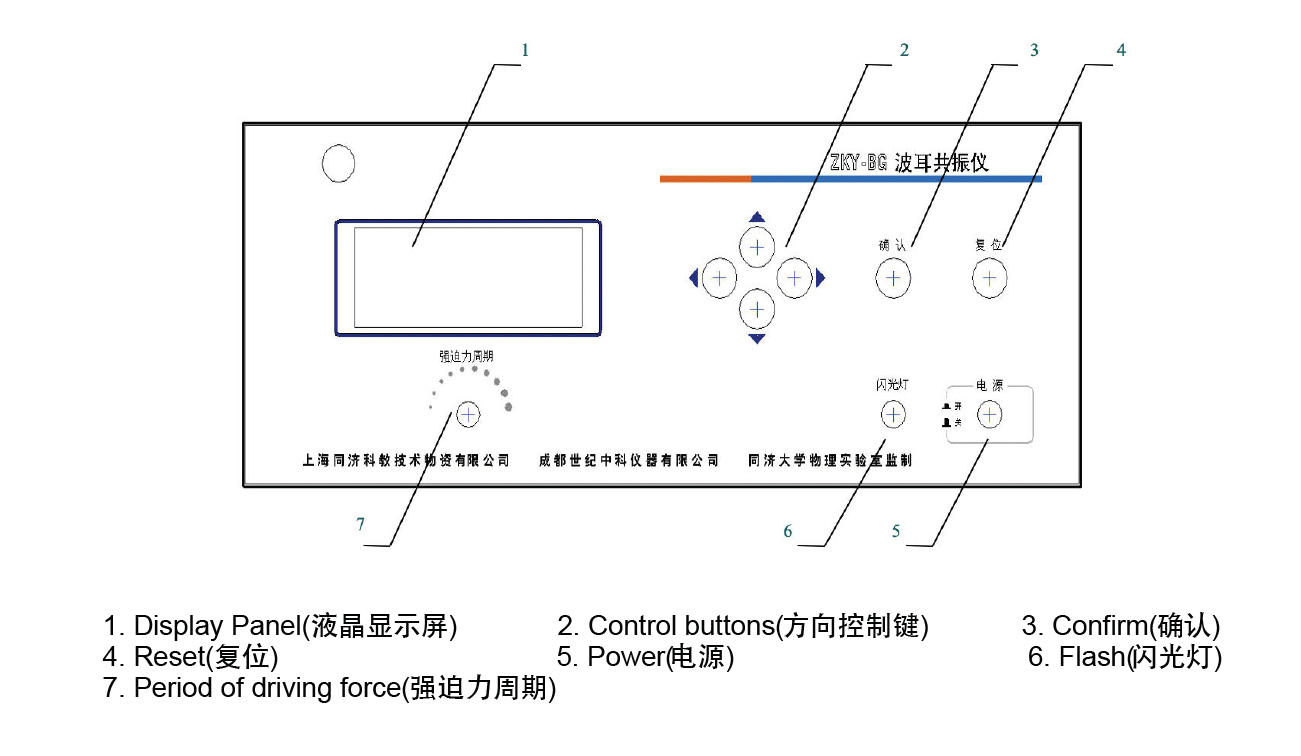
\includegraphics[width=10cm]{Front.png}
    \caption{The front panel of the control box}
\end{figure}

\section{Reference}
Qin Tian, Wang Yin, Tianyi Li, Mateusz Krzyzosiak, Physics Laboratory VP141 Exercise 5
Damped and Driven Oscillations. Mechanical Resonance

\section{Data Sheet and Uncertainty Data Sheet}

\end{document}